%!TEX root = ../thesis.tex

%%%%% Chapter: System Evaluation %%%%%
\chapter{System Evaluation}

\ifpdf
    \graphicspath{{Chapter7/Figs/Raster/}{Chapter7/Figs/PDF/}{Chapter7/Figs/}}
\else
    \graphicspath{{Chapter7/Figs/Vector/}{Chapter7/Figs/}}
\fi


\section{Overview}

\section{The Ground-Truth Data}

The ground-truth data of a single set of input lecture data (a handout PDF file + its associated audio file) can be seen as the correct mappings from the handout chunks (\texttt{BBoxGroup} objects) to the corresponding parts of the audio file (\texttt{TIntervalGroup} objects). The ground truth data as a whole can be represented by a \texttt{Matches} object described in \Cref{sec:basic-elem-matches}.

The ground-truth data should be labelled at the finest spatial scale possible, which means each \texttt{BBoxGroup} object in the ground-truth data is supposed to be as small (in its total area) as possible. This ensures the feasibility of the multi-scale evaluation of the alignment algorithm.

\section{Evaluating the Tesseract PLA}

Recall that the page layout analysis (PLA) of the Tesseract OCR engine produces a set of bounding-boxes which identifies distinct text regions in the PDF input. In \Cref{fig:eval-ocr-pla}, we can see how true positives (TP), true negatives (TN), false positives (FP) and false negatives (FN) are identified, given the bounding-boxes (a \texttt{BBoxGroups} object as a whole) in the ground-truth data. Here we assume that the bounding-boxes are non-overlapping for the ground-truth data and the OCR output respectively.

\begin{figure}[!htb]
    \centering
    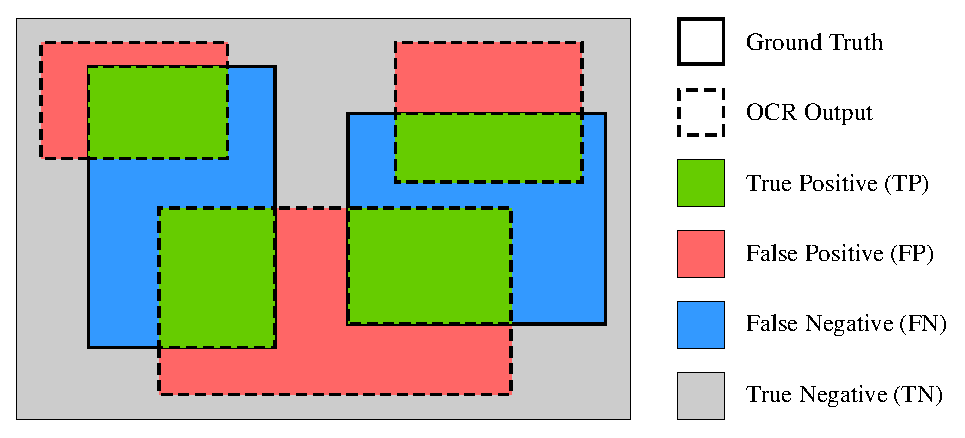
\includegraphics[width=0.75\textwidth]{eval-ocr-pla.eps}
    \caption{TP, TN, FP and FN in the evaluation of PLA}
    \label{fig:eval-ocr-pla}
\end{figure}

The key evaluation metrics are the \textit{true positive rate} (TPR) and \textit{true negative rate} (TNR), which are calculated as follows:
\[
    \begin{cases}
        \text{TPR \,=\, TP / (TP + FN)} \\
        \text{TNR =\, TN / (TN + FP)}
    \end{cases}
\]
Note that TPR is also called the recall rate. To calculate TPR and TNR, we sum up all rectangle areas for each certain type (TP, TN, FP and FN) and then substitute the values into the above equations.

The TPR (recall rate) essentially measures the fraction of the intersection area between the OCR output bounding-boxes and the bounding-boxes of the ground-truth data, with respect to the total area of the ground-truth bounding-boxes. The TNR, on the other hand, reflects how much useless area is included in the OCR output. Clearly we should maximise the TPR and minimise the TNR.